% !TEX root = main.tex
\documentclass[preprint,12pt]{elsarticle}

\usepackage{amsmath,amssymb}
\usepackage{booktabs}
\usepackage{graphicx}
\usepackage{multirow}
\usepackage{array}
\usepackage{url}
\usepackage{hyperref}
\makeatletter
\pdfstringdefDisableCommands{%
  \def\corref#1{}%
  \def\cnotenum#1{}%
  \def\@corref#1{}%
}
\makeatother
\usepackage{lineno}
\usepackage{microtype}
\emergencystretch=2em

\journal{Applied Energy}

\begin{document}

\begin{frontmatter}

\title{Distribution-shift-aware safe offline reinforcement learning for physics-constrained scheduling of regional integrated electricity--heat systems}

\author[a]{Pei He}
\ead{hepei002@mail.nwpu.edu.cn}

\author[b]{Haoyue Xue}
\ead{hxue8@illinois.edu}

\author[c]{Yangming Guo\corref{cor1}}
\ead{yangming\_g@nwpu.edu.cn}
\cortext[cor1]{Corresponding author}

\address[a]{School of Computer Science and Engineering, Northwestern Polytechnical University, Xi'an, Shaanxi 710072, China}
\address[b]{College of Agricultural, Consumer and Environmental Sciences, University of Illinois Urbana-Champaign, Urbana, IL 61801, USA}
\address[c]{School of Cybersecurity, Northwestern Polytechnical University, Xi'an 710072, China}

\begin{abstract}
Offline reinforcement learning (offline RL) can train fast dispatch policies without unsafe online exploration, but policies trained from fixed datasets may fail when regional integrated energy systems experience distribution shifts in load, weather, renewable availability or equipment parameters. This paper develops a distribution-shift-aware safe offline RL framework for physics-constrained electricity--heat scheduling. The framework combines CQL or IQL policies with a dynamics-ensemble out-of-distribution (OOD) risk estimator and an adaptive safety layer that passes, partially corrects or fully projects policy actions toward the physical feasible set. A reproducible case study is built from public German electricity, heat and weather time series for 2017--2019 and scaled to a medium-sized industrial park with 10 MW electric peak load and 18 MWth heat peak load. The experiments compare perfect-information optimization, rolling MPC, rule-based dispatch, behavior cloning, TD3+BC, raw CQL/IQL, fixed safety projection and adaptive safety under in-distribution, load-increase, cold-wave, equipment-fault and compound-stress scenarios. Raw CQL and IQL are fast but unsafe under severe shifts: in the cold-wave extreme scenario, their mean hard safety costs reach 49.93 and 58.21, respectively. Coupling them with the adaptive safety layer reduces the corresponding mean hard safety cost below numerical tolerance across the five-seed main experiments, with significant paired reductions in cold-wave, compound and load-up scenarios. The results show that OOD-aware physical correction can make offline RL dispatch more reliable under predefined shifts, while exposing the computation and intervention costs required for this reliability.
\end{abstract}

\begin{keyword}
Regional integrated energy system \sep electricity--heat scheduling \sep offline reinforcement learning \sep distribution shift \sep out-of-distribution risk \sep safe reinforcement learning \sep model predictive control
\end{keyword}

\end{frontmatter}

\section*{Highlights}
\begin{itemize}
  \item Offline RL scheduling is tested under electricity--heat distribution shifts.
  \item OOD risk is coupled with a physics-constrained adaptive safety layer.
  \item Public data build a reproducible three-year hourly RIES benchmark.
  \item Raw CQL and IQL show hard-safety failures under severe shifts.
  \item Adaptive safety reduces hard violations with explicit intervention costs.
\end{itemize}

\linenumbers

\section*{Nomenclature}

\small
\noindent\resizebox{0.95\textwidth}{!}{%
\begin{tabular}{ll}
\toprule
Symbol or term & Meaning \\
\midrule
RIES & Regional integrated energy system \\
Offline RL & Offline reinforcement learning trained from fixed trajectories \\
OOD risk & Out-of-distribution risk score for state--action pairs \\
CQL & Conservative Q-learning \\
IQL & Implicit Q-learning \\
MPC & Model predictive control \\
$s_t$ & State at hour $t$ \\
$a_t$ & Dispatch action at hour $t$ \\
$r_t$ & Economic reward at hour $t$ \\
$c_t$ & Safety cost at hour $t$ \\
$R_{\mathrm{OOD}}$ & OOD risk score \\
$\mathcal{F}$ & Physics-constrained feasible action set \\
$\Pi_{\mathcal{F}}$ & Safety projection operator \\
CHP & Combined heat and power \\
COP & Coefficient of performance \\
SOC & State of charge \\
CVaR & Conditional value-at-risk \\
\bottomrule
\end{tabular}
}

\section{Introduction}

Regional integrated energy systems (RIESs) are becoming a practical route for coordinating renewable electricity, heat production, flexible demand and storage at the district or industrial-park scale. In an electricity--heat RIES, photovoltaic generation, wind power, combined heat and power (CHP), heat pumps, batteries and thermal storage are not independent assets; their operating decisions are coupled through power balance, heat balance, equipment capacities, inter-temporal storage dynamics and reliability constraints. Integrated demand response, multi-energy coordination and data-driven energy-system operation can reduce operating cost and improve flexibility, but they also make dispatch sensitive to weather, load, energy-price and equipment-condition uncertainty \cite{Wang2017IntegratedDemandResponse,Ramprasad2022MLSustainableEnergy}.

Optimization-based dispatch methods, including deterministic optimization, robust or stochastic programming and model predictive control (MPC), remain natural tools for such systems because they represent physical constraints explicitly. Their practical performance, however, depends on the quality of forecasts, uncertainty sets and model parameters, and their repeated online solution may become burdensome as the system scale, time resolution and number of uncertainty scenarios increase. Reinforcement learning (RL) offers a complementary route: once trained, a policy can map the current system state to a dispatch action with very low online inference time. Yet conventional online RL is difficult to justify for safety-critical energy systems because exploration may violate supply, storage or equipment constraints \cite{Sutton1998RL,DulacArnold2021RealWorldRLChallenges}.

Offline reinforcement learning (offline RL) avoids online exploration by training policies from a fixed dataset of historical or simulated trajectories \cite{Levine2020OfflineRL,Prudencio2024OfflineRLSurvey}. This property makes offline RL especially appealing for energy management, where unsafe trial-and-error control is unacceptable. The central weakness is that the learned value function and policy are only reliable where the offline data provide sufficient support. When the deployed system experiences distribution shifts, such as cold waves, increased heat demand, renewable shortfalls, changed equipment efficiency or reduced interconnection capacity, an offline policy may select state--action pairs outside the training distribution. In an energy system, this is not merely a statistical inconvenience; it can lead to electric or thermal imbalance, storage state-of-charge violations, emergency load shedding or infeasible dispatch.

This paper studies safe offline RL for RIES scheduling from the perspective of distribution shift. Rather than evaluating only average in-distribution operating cost, we ask whether an offline policy remains physically reliable under load, weather, renewable, equipment and compound shifts, whether an out-of-distribution (OOD) risk score can identify dangerous state--action regions, and whether physical correction can reduce safety violations without turning the learned policy into an overly conservative optimizer. The proposed framework couples three components: an offline RL policy, a dynamics-ensemble OOD risk estimator, and an adaptive physics-constrained safety layer. The OOD score regulates how strongly the safety layer intervenes, ranging from pass-through to partial correction and full projection.

The contributions are threefold. First, we define a reproducible distribution-shift evaluation protocol for regional electricity--heat scheduling, covering in-distribution operation, load increase, renewable reduction, cold-wave/COP degradation, equipment degradation and compound stress. Second, we propose an OOD-aware adaptive safety mechanism that uses physical feasibility correction as a control action rather than as a post-hoc diagnostic. Third, we evaluate the method on a public-data-driven case study built from OPSD, When2Heat and weather time series \cite{OPSD2020TimeSeries,Moller2019When2Heat}, comparing optimization, MPC, rule-based control, multiple offline RL baselines, fixed safety correction and adaptive safety correction. The results show that unprotected offline RL can be fast but unsafe under severe shifts, whereas adaptive physics-constrained safety substantially reduces hard safety cost and tail risk. The scope is intentionally bounded: the paper studies an aggregated electricity--heat system and does not claim validated operation for detailed AC distribution networks, hydraulic thermal networks or real hardware controllers.

\section{Related work}

\subsection{Optimization and MPC for integrated energy dispatch}

Integrated energy dispatch has traditionally been formulated as an optimization problem with explicit physical constraints. Deterministic linear or mixed-integer programming models can represent energy balances, storage dynamics, CHP coupling and capacity limits, and open modelling tools such as PyPSA have made such constrained energy-system studies easier to reproduce \cite{Brown2018PyPSA}. Stochastic, scenario-based and robust formulations extend this structure to uncertainty in renewable generation, demand, flexibility and prices \cite{Parisio2022ScenarioStochasticMicrogrid,Zhang2020StochasticHybridSystem,Zhou2023GISStochasticMultiMicrogrid}. Multi-energy and multi-microgrid studies further show that coordination among electricity, heat, storage and networked microgrids can improve flexibility but introduces additional scheduling and communication complexity \cite{Mancarella2019MultiEnergyInfrastructureReview,Du2021MultiMicrogridEMSReview,Ahmad2023MicrogridEMSReview,Mashayekh2020OptimizationFrameworksMicrogrid,Zhang2024CollaborativeMultiEnergyMicrogrid}.

MPC provides a natural operational extension because it repeatedly solves a finite-horizon problem using updated measurements and forecasts. Building and energy-management reviews show that MPC can reduce energy cost and manage demand response when forecasts and models are reliable \cite{Drgona2020MPCBuildingsReview,Afram2021BEMSReview}. These approaches offer transparency and feasibility control, and they are strong baselines for any learning-based method. Their limitations in this paper are not conceptual but operational: repeated online optimization can be computationally costly, and performance depends on the accuracy of forecasts, uncertainty descriptions and model parameters.

\subsection{Reinforcement learning for energy management}

RL has been widely explored for building energy control, demand response, microgrid scheduling and multi-energy management because it can learn nonlinear policies and support fast online decisions after training \cite{VazquezCanteli2019DemandResponseRL,VazquezCanteli2021RLEnergySystems,Zhang2020RLModernPowerEnergy,Antonopoulos2020AIDemandResponseReview}. Representative studies cover whole-building HVAC control, home energy management, distributed microgrid markets, district energy management and RL--MPC hybrids \cite{Nagy2020RLHVACDemandResponse,Lee2021DRLHomeEnergy,Ye2020MARLHomeEnergy,Gao2020DeepComfort,Liu2021MADRMicrogridMarket,Nagy2021DistrictEnergyDRL,Drgona2022RLMPCBuilding}. Recent Applied Energy studies also examine hierarchical multi-agent energy management and safe DRL for building or multi-energy operation \cite{Liu2023MultiAgentHierarchicalRL,Yang2023PhysicalInformedSafeRL,Li2025SafeDRLBuildingEnergy}.

However, online RL assumes interaction with the environment and often relies on exploration, which is problematic for energy systems where unsafe actions can cause supply shortages or equipment violations. Comparisons between online/offline DRL and MPC in thermal energy management underline that learning-based control must be evaluated against model-based baselines rather than only against heuristic controllers \cite{Blad2022OnlineOfflineDRLMPC}. For regional electricity--heat dispatch, this means that safety cannot be assessed only through average reward; hard physical violations must be tracked as first-class outcomes.

\subsection{Offline reinforcement learning and distribution shift}

Offline RL trains from fixed datasets, making it more suitable for safety-critical operation than online exploration \cite{Levine2020OfflineRL,Prudencio2024OfflineRLSurvey}. Algorithms such as behavior cloning, TD3+BC \cite{Fujimoto2021TD3BC}, conservative Q-learning (CQL) \cite{Kumar2020CQL} and implicit Q-learning (IQL) \cite{Kostrikov2022IQL} attempt to reduce extrapolation error by constraining the learned policy or value function toward the dataset support. Broader reviews of real-world RL, model-based RL, transfer RL and zero-shot generalization show that deployment robustness depends on data coverage, model uncertainty and distributional change, not only on benchmark reward \cite{DulacArnold2021RealWorldRLChallenges,Moerland2023ModelBasedRLSurvey,Zhu2023TransferRLSurvey,Kirk2023ZeroShotDRLSurvey}.

Even so, the offline setting remains vulnerable to distribution shift. A dispatch policy trained from one range of load, weather and equipment conditions may not remain reliable when the deployed system moves outside that support. Uncertainty and OOD-detection surveys show that ensemble disagreement, novelty and predictive uncertainty can provide useful warning signals, but these signals are imperfect under rare-event imbalance \cite{Gawlikowski2023UncertaintyDNNSurvey,Yang2022OODDetectionReview,Ganaie2022EnsembleDeepLearningReview}. In the energy context, this weakness is amplified because unsafe extrapolation can translate directly into physical infeasibility. The gap addressed here is therefore not simply whether offline RL can imitate a good dispatcher, but whether its actions can be monitored and corrected when deployment conditions leave the data-supported region.

\subsection{Physics-informed safety layers}

A natural way to improve reliability is to couple learned actions with a model-based safety layer. Safe RL research has proposed shielding, barrier-function, chance-constrained and learning-based safety mechanisms for limiting unsafe exploration or unsafe control actions \cite{Garcia2015SafeRL,Brunke2022SafeLearningRobotics,Cheng2019SafeRLBarrierFunctions,Zhang2022SafeChanceConstrainedRL}. For an energy system, a safety layer can solve a minimum-correction problem that maps a candidate action toward the physical feasible set defined by power balance, heat balance, device limits and storage dynamics. This hybrid view retains the speed and flexibility of learning while preserving the interpretability of model-based feasibility correction.

The difficulty is that a fixed safety layer may intervene even when the learned action is already safe, thereby increasing operating cost or masking the contribution of the learned policy. Recent energy studies using physical-informed or safe RL show the value of embedding physical constraints, but they do not by themselves resolve how strongly a safety layer should intervene under changing data support \cite{Yang2023PhysicalInformedSafeRL,Li2025SafeDRLBuildingEnergy}. The adaptive mechanism proposed here addresses this issue by using OOD risk to regulate intervention strength.

\begin{table}[t]
\centering
\caption{Positioning of the proposed method relative to representative dispatch and learning paradigms.}
\label{tab:method_positioning}
\scriptsize
\setlength{\tabcolsep}{3pt}
\begin{tabular}{p{0.18\linewidth}p{0.25\linewidth}p{0.24\linewidth}p{0.18\linewidth}}
\toprule
Paradigm & Main strength & Main limitation for shifted RIES operation & Role in this paper \\
\midrule
Deterministic optimization & Explicit balances, device limits and storage dynamics & Requires accurate forecasts and repeated online solution & Perfect-information and feasibility reference \\
MPC / robust optimization & Updates decisions with forecasts and uncertainty descriptions & Performance depends on forecast quality, uncertainty sets and online solve time & Strong model-based baseline \\
Online RL & Fast policy after training and nonlinear control capability & Exploration can violate physical constraints during learning & Motivation for avoiding online exploration \\
Offline RL & Learns from fixed logs or simulations without online exploration & Vulnerable to extrapolation outside dataset support & Policy backbone tested under shifts \\
Safe RL / shielding & Adds constraints, safety filters or penalties to learned control & Safety treatment is often fixed or assumes online interaction & Conceptual basis for action correction \\
OOD-aware physical safety layer & Couples state--action risk with minimum physical correction & Requires a trusted aggregate model and adds correction cost & Proposed contribution \\
\bottomrule
\end{tabular}
\end{table}


\section{System model and problem formulation}

\subsection{Regional electricity--heat system}

The case study represents an aggregated medium-sized industrial park rather than a measured physical park. The system includes grid import and export, photovoltaic generation, wind generation, a gas CHP unit, an air-source heat pump, a lithium-ion battery, a thermal storage unit, electric load and heat load. The baseline scale is a 10 MW electric peak load and an 18 MWth heat peak load. The device capacities are summarized in Table~\ref{tab:system_parameters}. Technical parameter ranges are selected from public technology references where available \cite{EPA2015CHP,NREL2024BatteryATB}.

\begin{table}[t]
\centering
\caption{Main system scale and device parameters.}
\label{tab:system_parameters}
\small
\resizebox{\textwidth}{!}{%
\begin{tabular}{lll}
\toprule
Item & Value & Role/source \\
\midrule
Electric load peak & 10 MW & Scaled from German electricity load \\
Heat load peak & 18 MWth & Scaled from When2Heat heat demand \\
Grid import/export & 12 MW / 6 MW & Constrained interconnection \\
Photovoltaic & 6 MWp & Capacity-factor time series \\
Wind & 4 MW & Capacity-factor time series \\
CHP & 6 MWe / 7.2 MWth & Fixed heat-to-electric ratio 1.2 \\
Air-source heat pump & 10 MWth & Hourly COP from When2Heat \\
Battery & 4 MW / 8 MWh & SOC range 10--90\% \\
Thermal storage & 5 MW / 20 MWhth & SOC range 10--90\% \\
\bottomrule
\end{tabular}
}
\end{table}


At each hour $t$, the electricity balance relates grid exchange, renewable output, CHP electricity production, heat-pump electricity consumption, battery charge/discharge and electric load. The heat balance relates CHP heat production, heat-pump heat production, thermal storage charge/discharge and heat load. Renewable availability is treated as exogenous and curtailment is allowed. The heat pump COP is time-varying and derived from the heat-pump data source, so cold weather affects the system both by increasing heat load and by reducing heat-pump efficiency.

\subsection{Storage and device constraints}

Battery and thermal storage introduce inter-temporal dynamics. The battery has 8 MWh energy capacity, 4 MW charge/discharge power, 95\% charge and discharge efficiency, 0.0005 hourly self-discharge and a 10--90\% SOC range. The thermal store has 20 MWhth capacity, 5 MWth charge/discharge power, 95\% charge and discharge efficiency, 0.002 hourly heat loss and the same SOC range. Initial and terminal SOC are set to 50\% for the 24-hour dispatch horizon. The CHP is modeled with a fixed heat-to-electric ratio of 1.2 and a lower-heating-value electric efficiency of 0.40. The baseline model uses continuous operating variables without binary unit commitment, which keeps the deterministic dispatch, RL environment and safety projection mutually consistent.

\subsection{Markov decision process}

The scheduling problem is formulated as a finite-horizon Markov decision process with a 24-hour episode length and one-hour time step. The state $s_t$ contains normalized electric load, heat load, photovoltaic availability, wind availability, heat-pump COP, deterministic import-price signal, battery SOC, thermal-storage SOC and sinusoidal hour-of-day features. The import-price signal is a transparent time-of-use cost assumption used for dispatch evaluation and price-stress tests; it is not a claim of complete three-year historical day-ahead price coverage. The action $a_t$ is a four-dimensional normalized vector representing CHP electric output fraction, heat-pump heat-output fraction, signed battery power fraction and signed thermal-storage power fraction. The environment maps this action to physical dispatch variables and then enforces storage transitions, balance residuals and emergency slack accounting.

The reward is the negative one-hour operating cost, including grid import cost, gas cost, export revenue, curtailment penalties and emergency supply penalties. A separate hard safety cost $c_t$ records normalized physical infeasibility, including electricity and heat balance residuals, emergency electric or heat shedding, SOC-bound violations and device-limit residuals after dispatch. This index is reported separately from EUR operating cost because it measures physical reliability loss rather than money. Values below $10^{-6}$ are treated as numerical tolerance. This separation is important: a policy may have acceptable average economic cost but still be unacceptable if it violates hard physical constraints under rare conditions.

\subsection{Objective}

The practical objective is not to replace optimization in all settings, but to learn a fast dispatch policy that remains reliable under a predefined set of distribution shifts. We therefore evaluate policies by operating cost, hard safety cost, maximum violation, CVaR of cost or safety metrics, intervention rate, projection distance and decision time. A policy is considered useful only if it improves or preserves safety under shifted conditions without relying on unsupported claims of universal feasibility.

\begin{table}[t]
\centering
\caption{Evaluation metrics used to separate economics, safety, conservatism and computation.}
\label{tab:metric_definitions}
\small
\setlength{\tabcolsep}{4pt}
\begin{tabular}{p{0.23\linewidth}p{0.45\linewidth}p{0.22\linewidth}}
\toprule
Metric & Definition in the benchmark & Interpretation \\
\midrule
Episode operating cost & Sum of grid purchase, fuel and operating penalty terms over a 24-hour episode & Economic dispatch quality \\
Hard safety cost & Dimensionless normalized violation index aggregating electricity/heat balance residuals, emergency electric or heat shedding, SOC-bound residuals and device-limit residuals after dispatch; values below $10^{-6}$ are numerical tolerance & Physical reliability loss, not EUR cost \\
Maximum hard safety cost & Largest hourly hard safety cost within an episode & Worst within-day violation \\
CVaR of cost or safety & Mean value in the upper tail of episode-level cost or hard safety outcomes & Tail-risk exposure \\
Infeasible episode rate & Fraction of episodes with nonzero hard safety cost & Frequency of unacceptable dispatch \\
Projection distance & Euclidean distance between raw policy action and corrected action & Magnitude of physical correction \\
Intervention rate & Fraction of hours in which the safety layer changes the raw action & Conservatism and trust in the policy \\
Decision time & Mean wall-clock time for producing one dispatch action & Online computational burden \\
\bottomrule
\end{tabular}
\end{table}


\section{Distribution-shift-aware safe offline RL method}

\subsection{Offline policy learning}

Offline RL policies are trained from fixed datasets generated by behavior policies in the same physical simulation environment. The behavior policies include optimization-based and heuristic controllers, such as perfect-information optimization, rolling MPC, noisy MPC, rule-based control and safe random control. The resulting datasets represent expert, mixed and poor-quality coverage levels. The main offline RL algorithms are behavior cloning, TD3+BC, CQL and IQL, with CQL and IQL used as the principal policy backbones for the safety-layer experiments.

All offline policies use the same normalized state and action definitions. The training configuration uses a batch size of 256, hidden dimension 64, learning rate $5\times10^{-4}$, discount factor 0.99 and reward scale 0.001. The TD3+BC baseline uses a behavior-cloning weight of 2.5, CQL uses a conservatism coefficient of 0.5, and IQL uses expectile 0.7 with advantage temperature 3.0 and maximum advantage weight 20. These values are fixed before the reported shift evaluation rather than tuned per deployment scenario.

Offline training does not interact with the target deployment scenarios. This design reflects the intended safety-critical setting: the learning algorithm cannot explore arbitrary actions in the real energy system. It also creates the central risk studied in this paper, because the learned policy may face state--action combinations that are weakly represented in the offline data.

\subsection{Distribution-shift protocol}

The shift protocol defines a reference distribution and several shifted evaluation distributions. The reference distribution uses safe transitions from the expert offline dataset. The evaluation episodes are 24 hours long and are sampled from the 2019 evaluation period. The representative shift settings are summarized in Table~\ref{tab:shift_protocol}.

\begin{table}[t]
\centering
\caption{Representative distribution-shift scenarios used for evaluation. Relative changes are reported against the reference data.}
\label{tab:shift_protocol}
\small
\resizebox{\textwidth}{!}{%
\begin{tabular}{llrrrrr}
\toprule
Scenario & Family & $\Delta P^{load}$ & $\Delta Q^{load}$ & $\Delta PV$ & $\Delta Wind$ & $\Delta COP$ \\
\midrule
in\_distribution & baseline & 0.00 & 0.00 & 0.00 & 0.00 & 0.00 \\
load\_up\_20 & load & 0.20 & 0.20 & 0.00 & 0.00 & 0.00 \\
equipment\_degradation & equipment & 0.00 & 0.00 & 0.05 & 0.10 & 0.20 \\
cold\_wave\_extreme & weather\_extreme & 0.00 & 0.50 & 0.00 & 0.00 & 0.25 \\
compound\_extreme & compound\_extreme & 0.30 & 0.60 & 0.18 & 0.35 & 0.25 \\
\bottomrule
\end{tabular}
}
\end{table}


For generalization tests, additional cross-year, cross-season, climate-zone-inspired and compound stress scenarios are evaluated. These single-seed stress tests are used as robustness screening and failure-mode discovery, not as standalone inferential statistics.

\subsection{OOD risk estimation}

The OOD risk estimator is based on a dynamics ensemble. Each model takes a state--action pair and predicts the next-state increment. The risk score combines ensemble disagreement, mean prediction error and a state--action novelty term:
\begin{equation}
R_{\mathrm{OOD}} =
R_{\mathrm{disagreement}} +
R_{\mathrm{prediction\ error}} +
0.05 R_{\mathrm{novelty}} .
\end{equation}

The raw score is normalized using the 90th percentile of the training-set score. The adaptive layer uses low- and high-risk thresholds of 3.0 and 4.0, respectively, with an 11-point blend search between the raw and projected actions. The purpose of the OOD score is not merely to classify whether a point is outside the training distribution. Instead, it must be useful for energy dispatch: a high score should indicate increased likelihood of value error, projection distance, hard safety cost or performance degradation. In the implemented protocol, the global hard-safety discrimination of the ensemble OOD score reaches AUROC 0.708 and AUPRC 0.038, with an unsafe transition rate of 0.024. These values indicate a useful but imperfect signal; the score is therefore used to regulate safety intervention rather than to serve as the sole safety guarantee.

\subsection{Physics-constrained safety projection}

Given a raw policy action $a_t$, the safety projection solves a minimum-correction problem:
\begin{equation}
\tilde{a}_t = \Pi_{\mathcal{F}}(a_t)
= \arg\min_{a \in \mathcal{F}(s_t)} \|a-a_t\|_2^2 + \lambda \phi(a,s_t),
\end{equation}
where $\mathcal{F}(s_t)$ is the feasible set defined by electricity balance, heat balance, grid limits, CHP capacity and coupling, heat-pump COP relation, storage power and SOC limits, terminal SOC requirements and emergency supply variables. The function $\phi$ represents additional soft penalties used to discourage expensive or unreliable correction when multiple feasible actions are available. The projection is intended as a minimum physical correction, not as a full replacement for dispatch optimization.

The feasible set uses the same aggregate physical model as the deterministic dispatch baseline. Emergency electricity and heat shedding variables are included with high penalties, so the projection remains solvable while exposing infeasibility through the hard-safety metric. The projection is therefore a safety filter around the learned policy, not an unconstrained economic optimizer. This distinction matters for interpretation: feasibility restoration can come from the physical layer, while the learned policy is useful only when it reduces the amount or cost of correction needed to operate safely.

\subsection{Adaptive safety layer}

A fixed safety projection can reduce constraint violations but may become unnecessarily conservative. The adaptive safety layer uses the OOD risk score to regulate intervention. Let $r$ be the current OOD score and let $r_l$ and $r_h$ be low- and high-risk thresholds. The risk weight is
\begin{equation}
\rho =
\mathrm{clip}
\left(
\frac{r-r_l}{r_h-r_l},0,1
\right).
\end{equation}

When risk is low and the candidate action has no hard safety violation, the layer passes the action through. When risk is high, it applies the full physics-constrained projection. In the intermediate region, it searches for a feasible or near-feasible mixture between the raw action and the projected action, reducing unnecessary correction while preserving safety. The resulting controller can be summarized as
\begin{equation}
a_t^{\mathrm{safe}} =
\begin{cases}
a_t, & \rho \approx 0 \text{ and } a_t \text{ is safe},\\
(1-\alpha)a_t + \alpha \Pi_{\mathcal{F}}(a_t), & 0<\rho<1,\\
\Pi_{\mathcal{F}}(a_t), & \rho \approx 1.
\end{cases}
\end{equation}
The method therefore converts the OOD risk score into an operational decision: how much the learned policy should be trusted at the current state--action pair.

\begin{figure}[t]
  \centering
  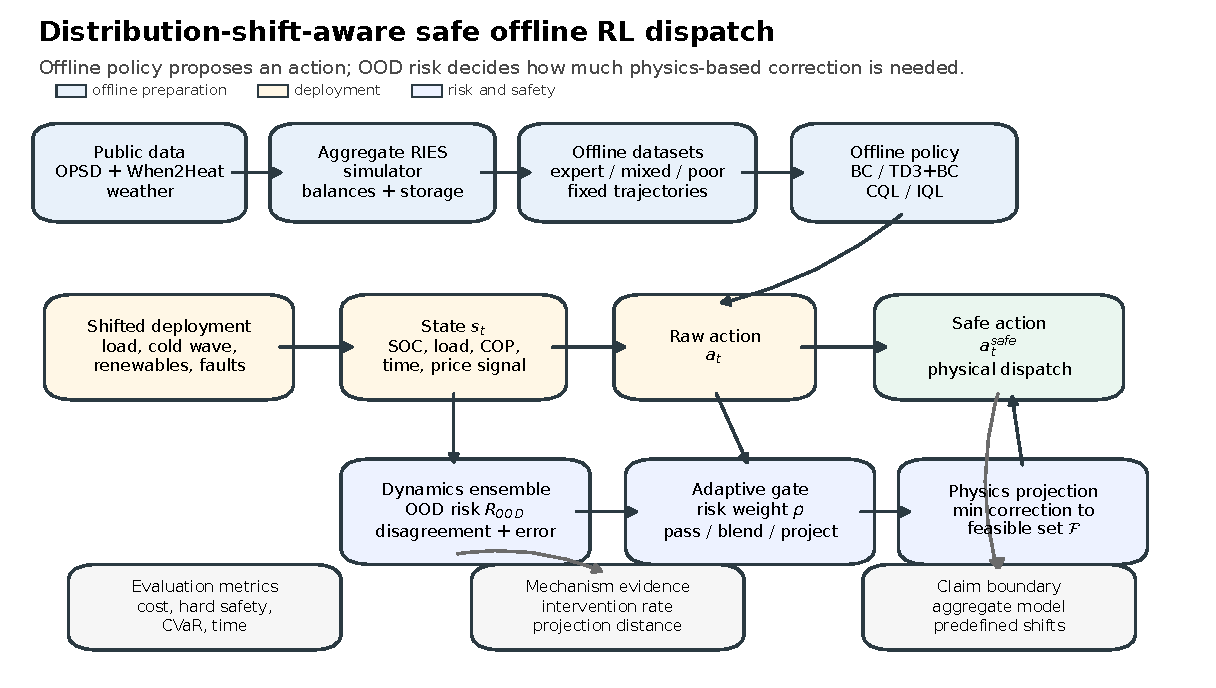
\includegraphics[width=0.95\linewidth]{../../results/figures/enhanced_manuscript/fig1_enhanced_framework.pdf}
  \caption{OOD risk is used as an action-level trust signal rather than only as a diagnostic. The framework separates offline preparation, shifted deployment, dynamics-ensemble OOD estimation, adaptive gating, physics-constrained projection and evaluation outputs, clarifying that the learned policy proposes an action while the physical layer restores modeled feasibility when needed.}
  \label{fig:framework}
\end{figure}

\section{Case study and experimental design}

\subsection{Data sources and preprocessing}

The exogenous time series are constructed from public sources. Electricity load, wind generation and photovoltaic generation are taken from OPSD time series \cite{OPSD2020TimeSeries}. Heat demand, domestic hot water and heat-pump COP information are taken from When2Heat \cite{Moller2019When2Heat,OPSD2023When2HeatDataset}. Weather-related variables are taken from OPSD Weather Data \cite{OPSD2020WeatherData}. The processed dataset is a complete hourly UTC-indexed table for 2017--2019. Daylight-saving time issues, duplicate timestamps and missing values are handled during preprocessing and recorded in the data provenance documentation. The German day-ahead price field is not used as a complete three-year input because it does not provide a common 2017--2019 window in the local data ledger; instead, dispatch costs use a deterministic time-of-use import-price profile and explicit price-multiplier stress tests.

The national-level time series are scaled to represent the simulated industrial park. Electric load is scaled to a 10 MW peak, and heat load is scaled to an 18 MWth peak. Photovoltaic and wind availability are converted to capacity factors and then applied to the 6 MWp PV and 4 MW wind capacities. This design creates a reproducible benchmark rather than a site-specific calibration.

\begin{figure}[t]
  \centering
  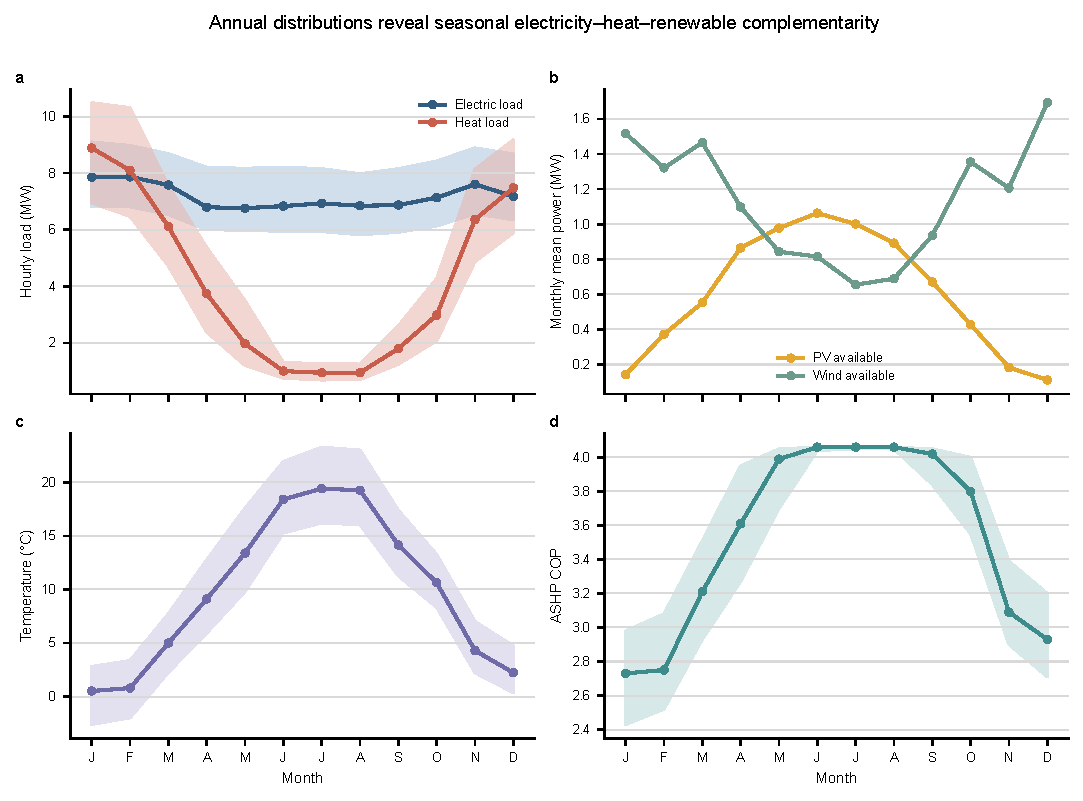
\includegraphics[width=0.95\linewidth]{../../results/figures/system_profiles/annual_distribution.pdf}
  \caption{The public-data benchmark contains seasonal and tail operating conditions that make average-case dispatch insufficient. The annual distributions of scaled electricity load, heat load, renewable availability and weather-derived variables define the operating envelope used for distribution-shift testing.}
  \label{fig:system_profiles}
\end{figure}

\subsection{Baselines}

The evaluated baselines are perfect-information linear programming, rolling MPC, rule-based control, behavior cloning, TD3+BC, CQL and IQL without safety correction, CQL and IQL with OOD warning only, CQL and IQL with fixed physics-constrained safety projection, and CQL and IQL with the proposed adaptive safety layer. The optimization and MPC baselines establish feasible model-based references. The rule-based controller tests whether learning is necessary. The unprotected offline RL baselines expose the effect of extrapolation under distribution shift. The fixed and adaptive safety variants isolate whether physical correction and risk-aware intervention improve the cost--safety trade-off.

\subsection{Evaluation scenarios and statistics}

The main multi-seed experiments include in-distribution operation, 20\% load increase, cold-wave extreme and compound extreme scenarios. CQL and IQL variants are evaluated over five random seeds. Additional stress tests include cross-year winter scenarios, summer peak, shoulder season, cold-climate-like and warm-low-solar-like scenarios, price-spike with low renewable output, cold wave with device fault and three-day low-renewable stress. These stress tests are included to reveal robustness boundaries.

The main economic metric is mean episode operating cost in EUR. The main safety metric is mean episode hard safety cost, supported by maximum hard safety cost, CVaR of hard safety cost, CVaR of episode cost and infeasible episode rate. The mechanism and conservatism metrics are projection distance and intervention rate. Computational efficiency is measured by mean decision time per step. For the five-seed scenarios, results are summarized using means, standard deviations and 95\% confidence intervals. Paired tests compare unprotected CQL/IQL against their adaptive safety variants and compare fixed safety against adaptive safety where seed-paired data are available. Single-seed stress-test $p$ values are not interpreted as statistical evidence.

\section{Results}

\subsection{OOD risk increases under safety-relevant shifts}

The distribution-shift protocol produces a clear ordering of risk across scenarios. The in-distribution scenario has a mean OOD score of 3.032 and zero unsafe transition rate in the rule-based evaluation sample. More severe scenarios increase both the OOD score and the observed safety risk. Load-up 20 has a mean OOD score of 3.373 and unsafe rate 0.010. Cold-wave extreme has a mean OOD score of 3.538 and unsafe rate 0.073. Compound extreme has a mean OOD score of 3.625 and unsafe rate 0.097. The global AUROC for hard-safety risk is 0.708. This result supports the use of the OOD score as an intervention signal, but it also reveals a limitation: the AUPRC is low because unsafe transitions are rare in the sampled protocol.

\begin{figure}[t]
  \centering
  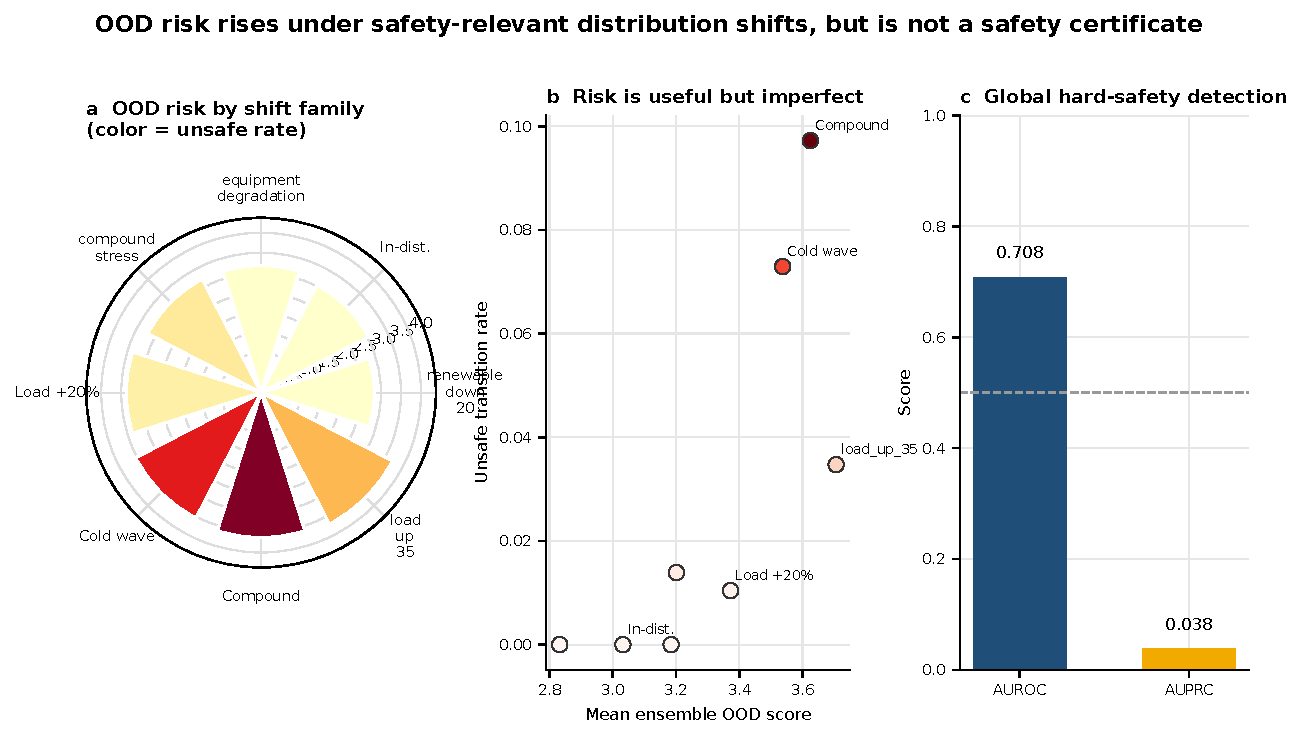
\includegraphics[width=0.95\linewidth]{../../results/figures/enhanced_manuscript/fig3_enhanced_ood_polar.pdf}
  \caption{OOD risk rises under the shifts that are most relevant to physical safety, but it is not a safety certificate. The polar risk map, risk--unsafe-rate scatter and global AUROC/AUPRC panel show that the ensemble score is useful as an intervention signal while remaining imperfect for rare unsafe-transition classification.}
  \label{fig:ood_summary}
\end{figure}

\subsection{Unprotected offline RL is fast but unsafe under major shifts}

Unprotected CQL and IQL policies have very low decision time, around 0.26 ms per step in the main experiments. However, their hard safety cost rises sharply under distribution shift. In the cold-wave extreme scenario, CQL reaches a mean episode cost of 414,519 EUR and mean hard safety cost of 49.93, while IQL reaches 480,323 EUR and mean hard safety cost of 58.21. In the compound extreme scenario, CQL reaches 538,233 EUR and hard safety cost of 64.49, while IQL reaches 620,851 EUR and hard safety cost of 74.89. Even in the load-up 20 scenario, CQL and IQL show hard safety costs of 12.55 and 20.12, respectively.

\begin{table}[t]
\centering
\caption{Main dispatch results. Costs are mean episode operating costs; hard safety cost summarizes physical infeasibility and emergency violations.}
\label{tab:main_results}
\scriptsize
\resizebox{\textwidth}{!}{%
\begin{tabular}{llrrrr}
\toprule
Scenario & Method & Cost (EUR) & Hard safety & Interv. rate & Time (ms) \\
\midrule
cold\_wave\_extreme & rolling\_mpc & 15402 & 0.00 & 0.00 & 7.71 \\
cold\_wave\_extreme & rule\_based & 17197 & 0.00 & 0.00 & 0.22 \\
cold\_wave\_extreme & cql & 414519 & 49.93 & 0.00 & 0.26 \\
cold\_wave\_extreme & cql\_adaptive\_safety & 16380 & 0.00 & 0.73 & 173.30 \\
cold\_wave\_extreme & iql & 480323 & 58.21 & 0.00 & 0.26 \\
cold\_wave\_extreme & iql\_adaptive\_safety & 16703 & 0.00 & 0.78 & 159.93 \\
compound\_extreme & rolling\_mpc & 22362 & 0.00 & 0.00 & 7.55 \\
compound\_extreme & rule\_based & 23221 & 0.00 & 0.00 & 0.19 \\
compound\_extreme & cql & 538233 & 64.49 & 0.00 & 0.26 \\
compound\_extreme & cql\_adaptive\_safety & 25089 & 0.00 & 0.78 & 146.49 \\
compound\_extreme & iql & 620851 & 74.89 & 0.00 & 0.27 \\
compound\_extreme & iql\_adaptive\_safety & 24536 & 0.00 & 0.83 & 142.91 \\
in\_distribution & rolling\_mpc & 11187 & 0.00 & 0.00 & 8.99 \\
in\_distribution & rule\_based & 13059 & 0.00 & 0.00 & 0.20 \\
in\_distribution & cql & 23991 & 1.27 & 0.00 & 0.26 \\
in\_distribution & cql\_adaptive\_safety & 13853 & 0.00 & 0.12 & 390.11 \\
in\_distribution & iql & 45034 & 3.93 & 0.00 & 0.28 \\
in\_distribution & iql\_adaptive\_safety & 13758 & 0.00 & 0.20 & 392.54 \\
load\_up\_20 & rolling\_mpc & 14945 & 0.00 & 0.00 & 7.99 \\
load\_up\_20 & rule\_based & 16655 & 0.00 & 0.00 & 0.19 \\
load\_up\_20 & cql & 117282 & 12.55 & 0.00 & 0.26 \\
load\_up\_20 & cql\_adaptive\_safety & 17374 & 0.00 & 0.60 & 228.54 \\
load\_up\_20 & iql & 177662 & 20.12 & 0.00 & 0.26 \\
load\_up\_20 & iql\_adaptive\_safety & 17343 & 0.00 & 0.70 & 192.74 \\
\bottomrule
\end{tabular}
}
\end{table}


\begin{figure}[t]
  \centering
  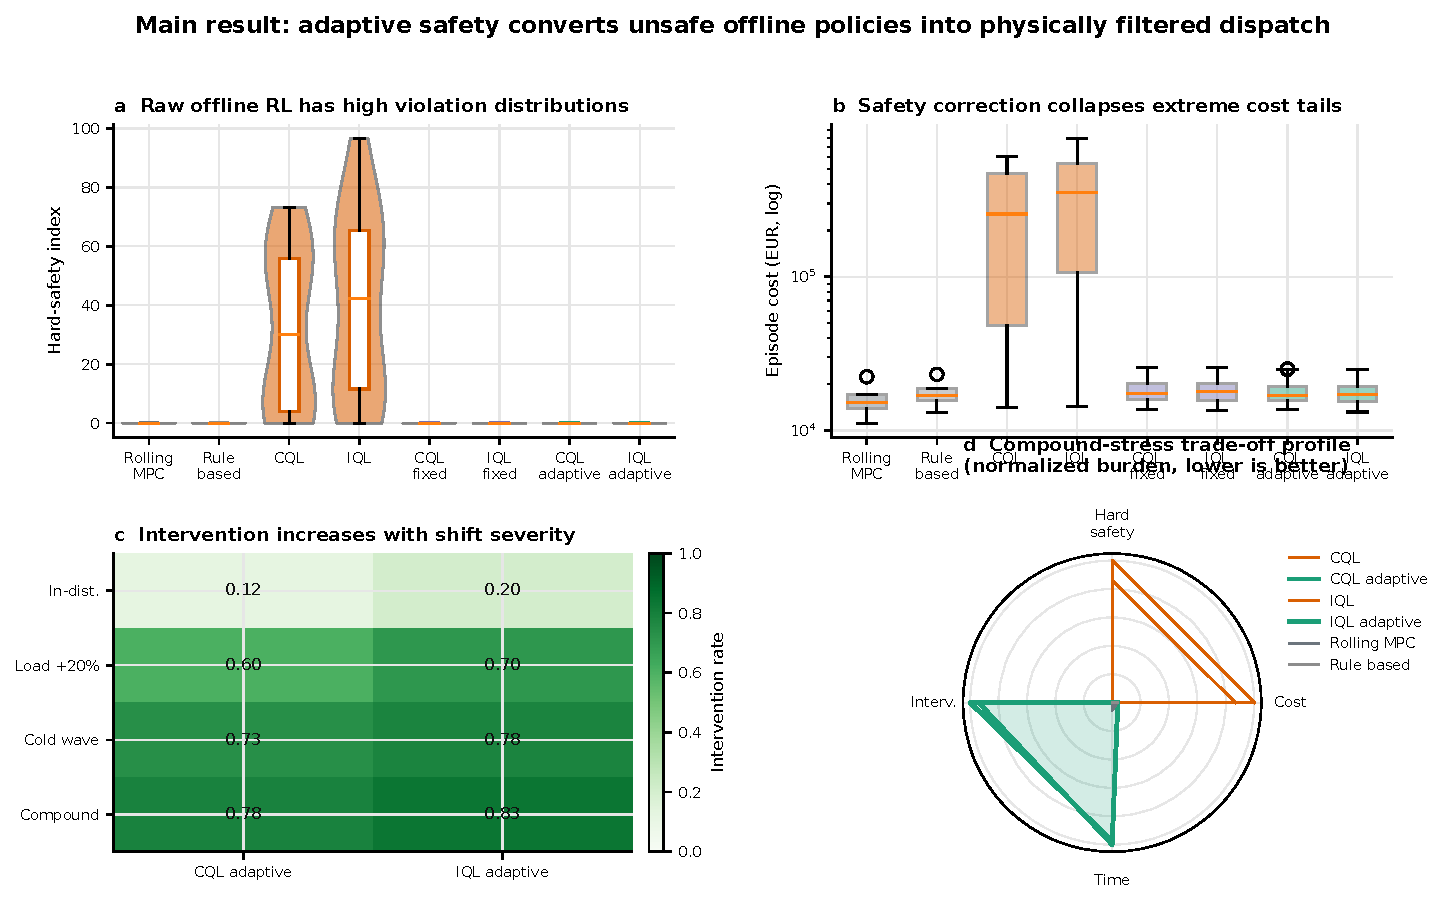
\includegraphics[width=0.95\linewidth]{../../results/figures/enhanced_manuscript/fig4_enhanced_main_violin.pdf}
  \caption{Raw offline RL is computationally fast but unsafe under shifted conditions, whereas adaptive safety reduces hard-safety cost below numerical tolerance in the five-seed main scenarios. Violin and box plots show the distribution of safety and cost outcomes, while the heatmap and radar panel summarize intervention intensity and compound-stress trade-offs.}
  \label{fig:main_results}
\end{figure}

\subsection{Adaptive safety removes hard violations in the main multi-seed scenarios}

Coupling CQL and IQL with the adaptive safety layer reduces mean hard safety cost below numerical tolerance in all four five-seed main scenarios. For CQL, the adaptive variant reduces mean hard safety cost from 49.93 to below tolerance in cold-wave extreme, from 64.49 to below tolerance in compound extreme, from 12.55 to below tolerance in load-up 20 and from 1.27 to zero in the in-distribution scenario. For IQL, the corresponding reductions are from 58.21, 74.89, 20.12 and 3.93 to below tolerance.

\begin{table}[t]
\centering
\caption{Paired tests for hard-safety reductions in five-seed scenarios. Negative mean delta indicates lower hard safety cost after adaptive safety.}
\label{tab:paired_tests}
\small
\resizebox{\textwidth}{!}{%
\begin{tabular}{llrrr}
\toprule
Scenario & Comparison & Pairs & Mean delta & $p$ value \\
\midrule
cold\_wave\_extreme & iql $\rightarrow$ iql\_adaptive\_safety & 5 & -58.21 & 0.0005 \\
cold\_wave\_extreme & cql $\rightarrow$ cql\_adaptive\_safety & 5 & -49.93 & 0.0001 \\
compound\_extreme & iql $\rightarrow$ iql\_adaptive\_safety & 5 & -74.89 & 0.0002 \\
compound\_extreme & cql $\rightarrow$ cql\_adaptive\_safety & 5 & -64.49 & 0.0000 \\
load\_up\_20 & iql $\rightarrow$ iql\_adaptive\_safety & 5 & -20.12 & 0.0168 \\
load\_up\_20 & cql $\rightarrow$ cql\_adaptive\_safety & 5 & -12.55 & 0.0094 \\
\bottomrule
\end{tabular}
}
\end{table}


The paired tests support these reductions in the shifted multi-seed scenarios. For cold-wave extreme, the adaptive layer reduces hard safety cost relative to IQL by 58.21 with $p=0.00051$, and relative to CQL by 49.93 with $p=0.000098$. For compound extreme, the reductions are 74.89 for IQL with $p=0.000196$ and 64.49 for CQL with $p=0.000032$. For load-up 20, the reductions are 20.12 for IQL with $p=0.0168$ and 12.55 for CQL with $p=0.00938$.

\subsection{Adaptive safety trades computation and intervention for reliability}

The reliability gain is not free. Adaptive safety increases decision time relative to raw offline RL because the safety layer must evaluate risk and solve or approximate a physical correction. In the main experiments, CQL adaptive safety requires approximately 146--390 ms per step depending on scenario, while raw CQL requires about 0.25--0.26 ms. IQL adaptive safety requires approximately 143--393 ms per step, while raw IQL requires about 0.26--0.28 ms.

The intervention rate also reflects scenario severity. For CQL adaptive safety, the intervention rate is 0.117 in distribution, 0.600 for load-up 20, 0.733 for cold-wave extreme and 0.783 for compound extreme. For IQL adaptive safety, the corresponding rates are 0.200, 0.700, 0.775 and 0.833. This ordering is consistent with the intended behavior: the layer intervenes more often when the environment is shifted and the raw policy action is more likely to be unsafe.

\subsection{Adaptive correction reduces conservatism relative to fixed projection}

Both fixed and adaptive safety variants reduce hard safety cost to numerical tolerance in the main scenarios. This result is useful but also limits the safety claim: the adaptive layer should not be interpreted as the only source of feasibility. The physical projection is the component that restores modeled feasibility, while the OOD-adaptive mechanism determines how much correction is applied.

\begin{table}[t]
\centering
\caption{Trade-off between fixed and OOD-adaptive safety correction in the five-seed main scenarios. Both variants reduce hard-safety cost to numerical tolerance; the adaptive layer mainly reduces operating cost and correction magnitude rather than being the sole source of feasibility.}
\label{tab:fixed_adaptive_tradeoff}
\scriptsize
\resizebox{\textwidth}{!}{%
\begin{tabular}{llrrrrrrrrr}
\toprule
Scenario & Policy & Fixed cost & Adaptive cost & $\Delta$ cost & Fixed interv. & Adaptive interv. & Fixed dist. & Adaptive dist. & Fixed time & Adaptive time \\
 & & (EUR) & (EUR) & (EUR) & & & & & (ms) & (ms) \\
\midrule
in\_distribution & CQL & 13944 & 13853 & -91 & 0.11 & 0.12 & 0.036 & 0.014 & 405.0 & 390.1 \\
load\_up\_20 & CQL & 18159 & 17374 & -785 & 0.60 & 0.60 & 0.364 & 0.154 & 215.7 & 228.5 \\
cold\_wave\_extreme & CQL & 16715 & 16380 & -335 & 0.73 & 0.73 & 0.543 & 0.477 & 151.8 & 173.3 \\
compound\_extreme & CQL & 25521 & 25089 & -432 & 0.78 & 0.78 & 0.661 & 0.574 & 129.1 & 146.5 \\
in\_distribution & IQL & 13875 & 13758 & -117 & 0.20 & 0.20 & 0.064 & 0.036 & 385.0 & 392.5 \\
load\_up\_20 & IQL & 18143 & 17343 & -800 & 0.70 & 0.70 & 0.440 & 0.229 & 172.6 & 192.7 \\
cold\_wave\_extreme & IQL & 17332 & 16703 & -629 & 0.78 & 0.78 & 0.629 & 0.506 & 146.1 & 159.9 \\
compound\_extreme & IQL & 24885 & 24536 & -349 & 0.83 & 0.83 & 0.737 & 0.661 & 116.2 & 142.9 \\
\bottomrule
\end{tabular}
}
\end{table}


Table~\ref{tab:fixed_adaptive_tradeoff} shows that the adaptive layer mainly improves the cost--correction trade-off. For CQL, adaptive safety lowers mean operating cost relative to fixed safety by 91--785 EUR across the four main scenarios and reduces projection distance in all four cases. For IQL, the corresponding cost reduction is 117--800 EUR, again with lower projection distance in all four cases. The intervention rate is similar because both variants must correct unsafe actions under shifted conditions; the difference is that the adaptive blend changes the magnitude of correction. The additional computation is scenario dependent, ranging from a small reduction in the in-distribution CQL case to a higher cost in the shifted cases. These results support a bounded interpretation: OOD-adaptive safety improves how the projection is used, rather than replacing the need for a trusted physical model.

This distinction is important for the contribution of the paper. A fixed projection answers the binary question of whether a candidate action should be corrected to the feasible set. The proposed adaptive layer answers a more operational question: how much of the learned action should be trusted under the current state--action support. In low-risk regions, the learned action can be retained or only weakly corrected; in high-risk regions, the same physical projection becomes a stronger safeguard. The value of the OOD signal is therefore not that it alone certifies safety, but that it reduces unnecessary correction when the offline policy remains close to the data-supported operating envelope while still allowing full projection under severe shifts. This is the main mechanism by which the method improves the cost--correction trade-off relative to fixed safety.

\subsection{Ablation, stress tests and failure modes}

\begin{figure}[t]
  \centering
  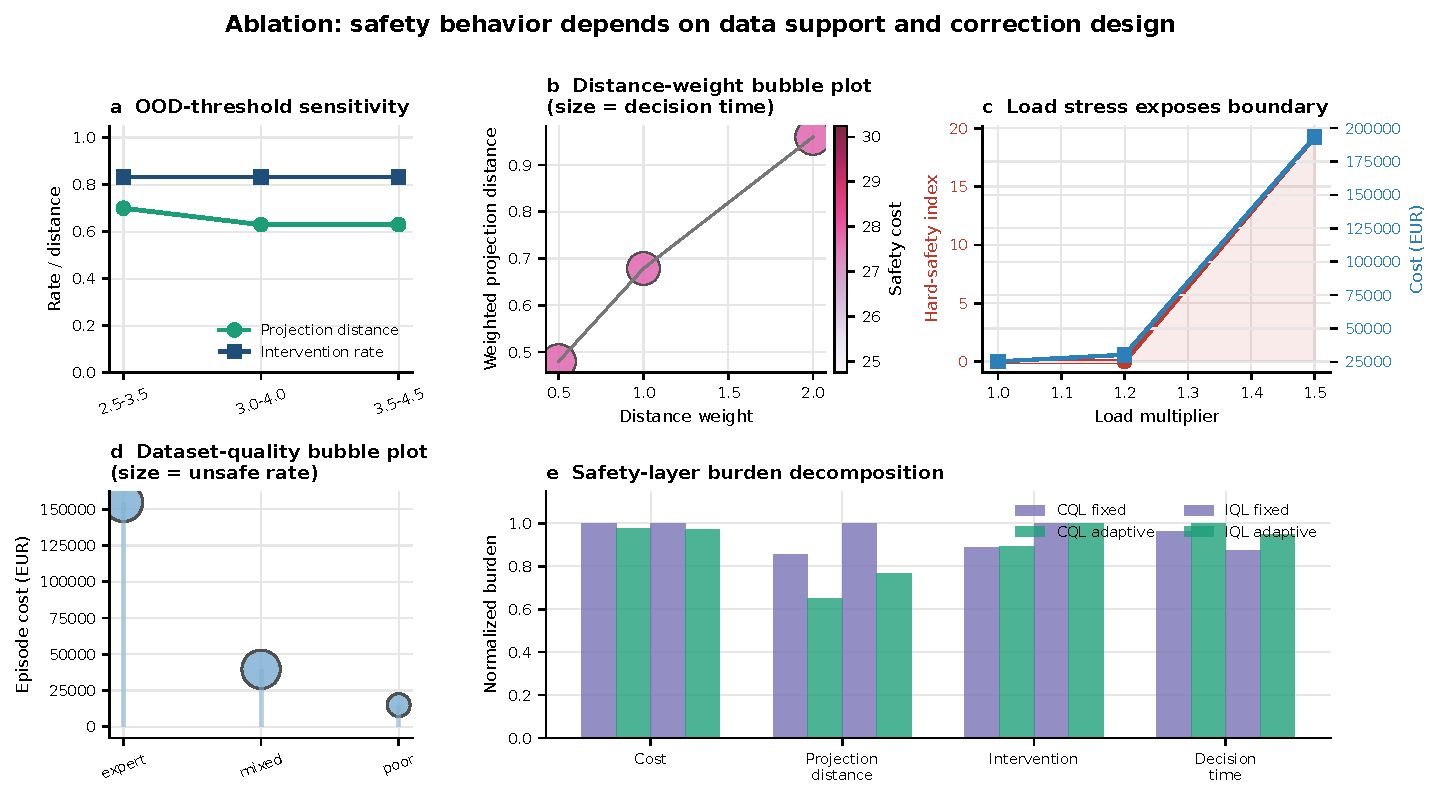
\includegraphics[width=0.95\linewidth]{../../results/figures/enhanced_manuscript/fig5_enhanced_ablation_heatmap.pdf}
  \caption{The safety behavior is not explained by a single favourable dataset or parameter choice. Threshold curves, distance-weight bubbles, load-stress response, data-quality bubbles and safety-layer burden decomposition show how data support and correction design affect the cost--safety--conservatism trade-off.}
  \label{fig:ablation}
\end{figure}

The Week 15 stress tests extend the evaluation beyond the four main scenarios. Under cold-climate, cross-year winter, price-spike, device-fault and low-renewable stress conditions, unprotected CQL and IQL can again show nonzero hard safety cost, whereas adaptive safety variants reduce hard safety cost below numerical tolerance in the recorded single-seed runs. Because these stress tests are single-seed evaluations, they support qualitative robustness screening and failure-mode discovery rather than independent statistical proof.

\begin{figure}[t]
  \centering
  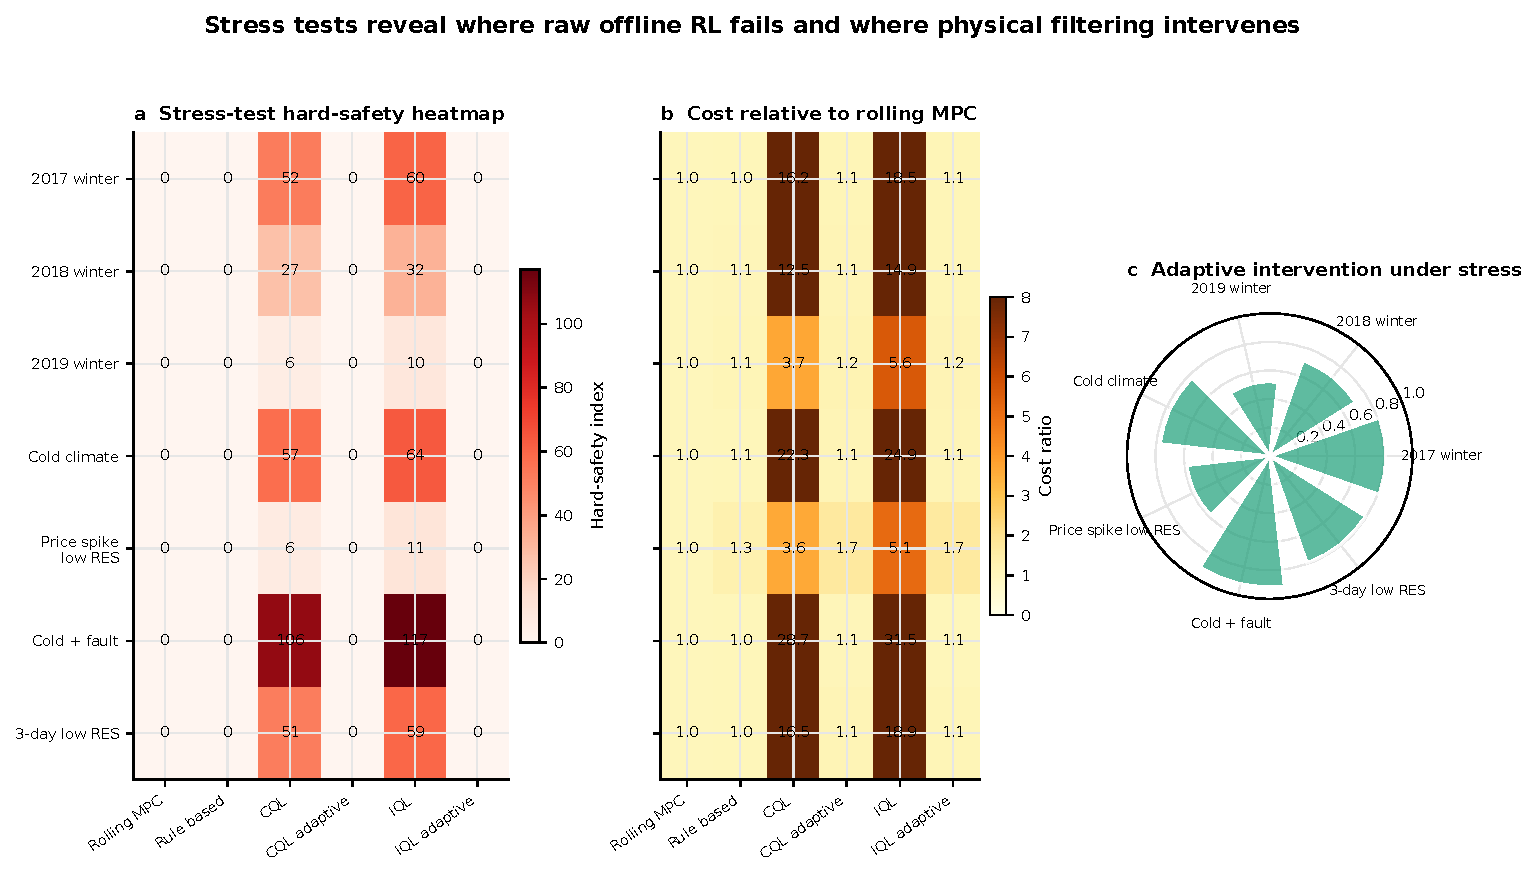
\includegraphics[width=0.95\linewidth]{../../results/figures/enhanced_manuscript/fig6_enhanced_stress_heatmap.pdf}
  \caption{Stress tests expose the boundary of the method rather than serving as independent statistical proof. The hard-safety heatmap, cost-ratio heatmap and polar intervention map show where unprotected offline RL can fail and where adaptive safety still restores modeled feasibility in recorded single-seed runs.}
  \label{fig:stress}
\end{figure}

\begin{figure}[t]
  \centering
  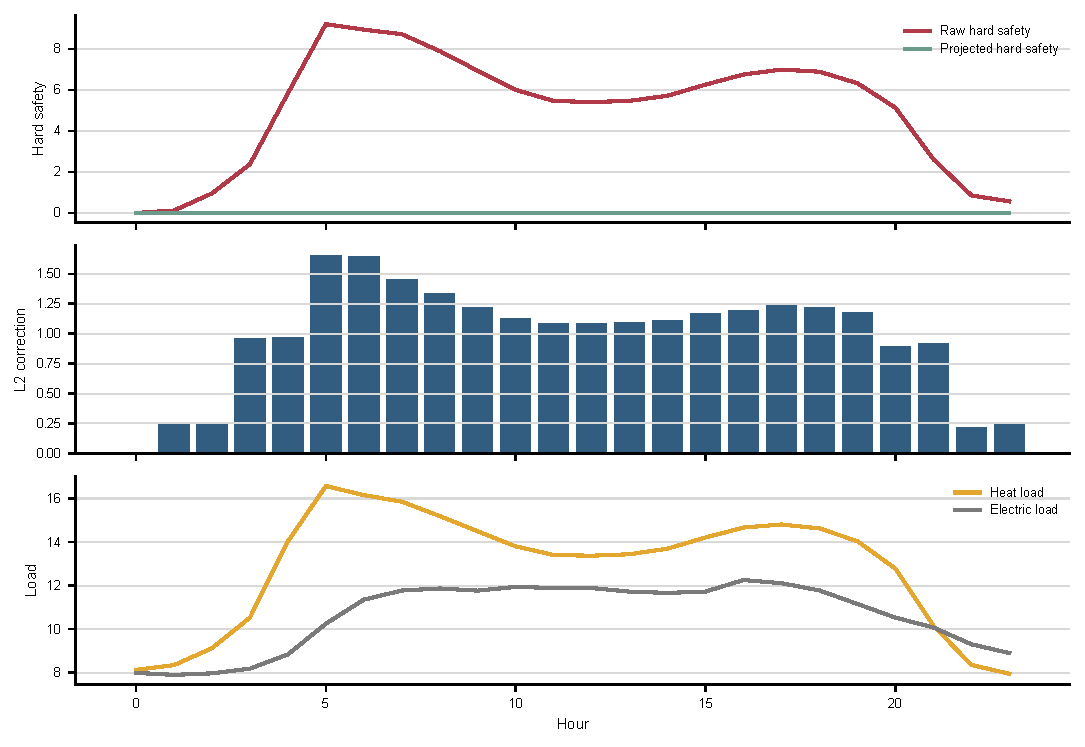
\includegraphics[width=0.95\linewidth]{../../results/figures/week15_16/week15_intervention_trajectory.pdf}
  \caption{Adaptive intervention concentrates at the hours where the raw policy becomes least trustworthy. The trajectory links OOD risk, intervention decisions and hard-safety reduction in a representative stress episode, illustrating the mechanism behind the aggregate safety results.}
  \label{fig:trajectory}
\end{figure}

\begin{figure}[t]
  \centering
  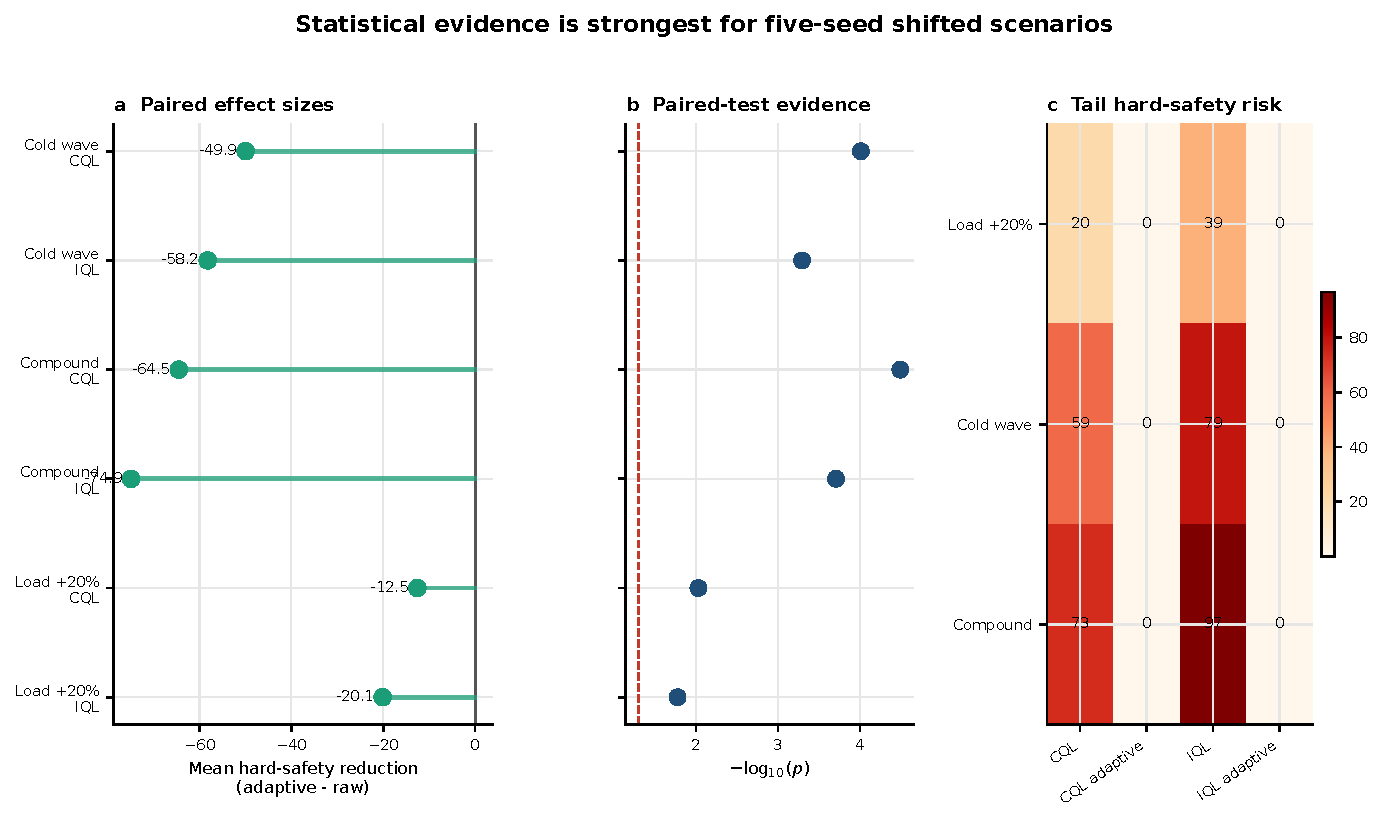
\includegraphics[width=0.95\linewidth]{../../results/figures/enhanced_manuscript/fig8_enhanced_statistics_forest.pdf}
  \caption{Only the five-seed scenarios support inferential comparisons, while single-seed stress scenarios diagnose failure modes. The forest-style effect-size panel, paired-test evidence and tail-risk heatmap separate robust statistical evidence from boundary-screening evidence.}
  \label{fig:statistics}
\end{figure}

\section{Discussion}

\subsection{Policy learning and physical correction play different roles}

The results indicate that the main weakness of offline RL in this setting is not average in-distribution economic performance but shifted-condition safety. Raw CQL and IQL can choose actions quickly, but their learned value functions and action distributions do not by themselves enforce electricity--heat feasibility. When cold weather, heat demand, COP degradation or compound stress moves the system away from the training support, the learned policy can produce actions that require infeasible balancing or emergency correction.

The physical projection and the learned policy therefore play different roles. The projection supplies modeled feasibility with respect to the aggregate electricity--heat constraints. The offline policy supplies a candidate dispatch action that may reduce cost or correction effort when the state--action pair remains close to the data-supported region. The adaptive OOD mechanism links these roles by reducing trust in the learned action when the ensemble risk score increases. This means that the method should be read as an OOD-aware safety-filter architecture, not as evidence that an unconstrained offline RL policy is intrinsically safe.

\subsection{Relation to optimization-based control}

The proposed method should be viewed as a hybrid learning-control architecture rather than a replacement for optimization. Perfect-information optimization and rolling MPC remain essential references because they provide physically feasible dispatch under known model assumptions. The rule-based controller is also a strong baseline in this aggregate benchmark, which is why the paper does not claim that offline RL dominates simple operational heuristics. The contribution is narrower: the experiments expose how raw offline RL fails under distribution shift and show how a risk-aware physical filter can restore modeled feasibility while reporting the intervention and correction costs required to do so.

The computation results also set a practical boundary. In this benchmark, the safety layer can be computationally heavier than raw policy inference and, in some measured cases, heavier than the small rolling MPC implementation. This finding prevents an exaggerated claim that safe offline RL is automatically faster than MPC. A stronger future implementation may exploit warm starts, analytical projections or reduced-order constraints to improve real-time performance. Until such acceleration is demonstrated, the method is most credible as an advisory controller or safety filter evaluated against MPC, rather than as a blanket replacement for online optimization.

\subsection{What the OOD score does and does not prove}

The dynamics-ensemble OOD score provides a graded risk signal, with higher scores in cold-wave and compound stress scenarios. The global AUROC above 0.70 suggests useful discrimination, but the low AUPRC shows that rare unsafe transitions remain hard to identify precisely. Therefore, the OOD score should not be used as a standalone certificate of safety. Its role is operational: to modulate a physical correction mechanism that can directly enforce or restore feasibility. This distinction is central to the paper. The novelty is not only detecting that a policy may be outside distribution, but connecting that signal to a physics-aware action correction.

From an energy-system perspective, this imperfect but monotone risk signal is still useful because the control consequence is asymmetric. A false high-risk warning mainly increases correction distance and operating conservatism, whereas an uncorrected high-risk action can create electric or thermal imbalance. The adaptive layer therefore treats the ensemble score as a trust indicator rather than as a classifier with a hard alarm threshold. The reported AUROC, AUPRC, intervention rates and threshold ablations should be interpreted together: they show that the score is not sufficient as a rare-event detector by itself, but is informative enough to allocate physical correction effort across in-distribution, load-up, cold-wave and compound-stress cases.

\subsection{Implications for resilient electricity--heat park operation}

The case study is simulated, but the stress factors are operationally meaningful for regional electricity--heat systems. Cold waves can simultaneously increase heat demand and reduce heat-pump COP; renewable shortfalls reduce local supply; equipment degradation changes feasible operating margins; and compound events combine these effects. In such conditions, a learned policy may still provide useful candidate actions, but operators need to know when the learning component is being trusted and when the physical model is taking over. The proposed architecture provides three diagnostic quantities for this purpose: the OOD risk score, the intervention rate and the projection distance. These quantities can be used as supervisory signals in an operator-advisory setting, as triggers for fallback operation, or as stress-test indicators during controller validation.

The practical message is therefore not that offline RL should replace MPC or rule-based operation. Rather, offline RL can be made more credible for safety-critical scheduling when it is embedded in a transparent risk-aware safety filter. This framing is consistent with integrated energy-system operation, where physical feasibility, reliability margins and operator interpretability are at least as important as average operating cost.

\subsection{Limitations and practical implications}

The study has several boundaries. First, the case study is an aggregated simulated industrial park calibrated from public time series, not a measured closed-loop field experiment or a site-calibrated industrial dataset. Second, the physical model omits detailed AC power flow, thermal-network hydraulics, gas-network dynamics, binary unit commitment and hardware-control delays. Third, the offline datasets are generated from simulated behavior policies rather than real operator logs. Fourth, the price signal is a deterministic time-of-use cost assumption, with price spikes treated as stress tests rather than historical market replay. Fifth, the stress-test scenarios are predefined; they do not cover arbitrary structural failures or adversarial events. Sixth, some generalization tests are single-seed and should be interpreted as robustness screening.

For practitioners, the results suggest a cautious path for using learning-based dispatch in safety-critical energy systems. Offline RL should not be deployed as an unconstrained action generator under uncertain conditions. A more credible design is to combine learned policies with risk monitoring and model-based feasibility correction. Such a controller can use learning where data support is strong and rely more heavily on physical correction when the state--action pair becomes unusual. This design also creates useful diagnostic outputs, including OOD score, intervention rate and projection distance, which can help operators understand when the learning component is being trusted.

\section{Conclusions}

This paper developed a distribution-shift-aware safe offline reinforcement learning framework for physics-constrained scheduling of a regional integrated electricity--heat system. The framework combines offline RL policies, a dynamics-ensemble OOD risk estimator and an adaptive physical safety layer that regulates action correction according to risk. A public-data-driven case study for 2017--2019 was constructed for a medium-sized industrial park with coupled electricity and heat assets.

The experiments show that unprotected offline RL policies can be computationally fast but unsafe under severe load, weather and compound shifts. In the five-seed main experiments, adaptive safety reduces the mean hard safety cost of CQL and IQL below numerical tolerance in cold-wave, compound and load-up scenarios, with paired tests showing significant reductions relative to the unprotected policies. The adaptive layer also provides a measurable intervention signal: correction frequency and projection distance increase under more severe shifts. These results support the use of OOD-aware physical correction as a candidate safeguard for offline RL dispatch.

The study also clarifies the boundary of the claim. The proposed method is not a universal safety certificate, and the current projection implementation has nontrivial computation cost. Future work should integrate network-constrained power and heat-flow models, validate the method with real operation logs or hardware-in-the-loop simulation, improve projection speed, and extend the distribution-shift protocol to multi-park coordination and market interaction.

\section*{Data and code availability}

This study reuses public third-party datasets rather than measured proprietary park data. Electricity load, wind and photovoltaic time series were obtained from OPSD Time Series version 2020-10-06 \cite{OPSD2020TimeSeries}. Weather variables were obtained from OPSD Weather Data version 2020-09-16 \cite{OPSD2020WeatherData}. Heat-demand and heat-pump COP inputs were obtained from When2Heat version 2023-07-27 and its data descriptor \cite{Moller2019When2Heat,OPSD2023When2HeatDataset}. Historical German day-ahead prices are not included in the processed three-year benchmark because the local OPSD field does not provide a complete common 2017--2019 window; deterministic time-of-use prices and price multipliers are used only as transparent cost assumptions. The reported benchmark does not use ERA5 fields; ERA5 is reserved for possible future spatial or post-2019 extensions.

The authors processed these sources into a complete hourly UTC-indexed Germany benchmark for 2017--2019, with daylight-saving-time transitions, duplicate timestamps and missing values handled as described in the preprocessing documentation. The code, configuration files, processed benchmark table, offline datasets, result tables, manuscript figure files and LaTeX source are available at \url{https://github.com/hepei002/safe-offline-rl-ries-dispatch}. A release DOI or accession will be added after archiving the final submission snapshot in a persistent repository. Raw third-party datasets should be cited and obtained from their original providers, because redistribution and attribution conditions are governed by the corresponding OPSD and When2Heat records.

\section*{Funding}

This work was supported by the Zhejiang Provincial Excellent Funding for Postdoctoral Researchers (Grant No. ZJ2025156) and the China Postdoctoral Science Foundation (Grant No. 2025M784428).

\section*{CRediT authorship contribution statement}

Pei He: Conceptualization, Methodology, Software, Validation, Formal analysis, Data curation, Writing -- original draft, Visualization, Funding acquisition. Haoyue Xue: Methodology, Validation, Formal analysis, Writing -- review \& editing. Yangming Guo: Supervision, Project administration, Writing -- review \& editing.

\section*{Declaration of competing interest}

The authors declare that they have no known competing financial interests or personal relationships that could have appeared to influence the work reported in this paper.

\section*{Declaration of generative AI and AI-assisted technologies in the writing process}

During the preparation of this work, the authors used AI-assisted writing tools to organize text from local project documents, result tables and manuscript notes. The authors reviewed and edited the content and take full responsibility for the content of the publication.
\bibliographystyle{elsarticle-num}
\bibliography{references}

\end{document}

